% ===========================================================================
% main.tex — the ORCHESTRATOR. This file owns the preamble and the order of
% the paper; it holds no prose itself. Everything is pulled in with \input{}.
%
% Two kinds of inputs, two workflows:
%
%   sections/*.tex        PROSE, no data. Live-edit these on Overleaf with
%                         co-authors. Pull their edits back into git.
%
%   output/tabs/*.tex     GENERATED from data by R/03_analysis.R. Render and
%   ../figures/*.png      push them; never hand-edit. Re-run the script and
%                         they update on the next compile.
%
% This split keeps collaboration (prose) and reproducibility (data) from
% stepping on each other, while one file keeps the overview of the whole paper.
% ===========================================================================
\documentclass[11pt]{article}

\usepackage[a4paper, margin=1in]{geometry}
\usepackage[utf8]{inputenc}
\usepackage{graphicx}
\usepackage{natbib}
\usepackage{booktabs}
\usepackage{hyperref}

\title{Framing effects on consumer purchase intention: \\
       a mediation and moderation analysis}
\author{Your Name}
\date{\today}

\begin{document}
\maketitle

\begin{abstract}
% sections/abstract.tex — PROSE (no data). Safe to live-edit on Overleaf.
We test whether messaging frames (scarcity, sustainability, social proof,
and a combined frame) increase purchase intention for everyday consumer
products, whether this effect is mediated by perceived value, and whether
it is moderated by price sensitivity. Data, scripts, and outputs live in
the same git repository as this manuscript.

\end{abstract}

% ---- Prose sections (live-editable on Overleaf) ---------------------------
% sections/introduction.tex — PROSE (no data). Safe to live-edit on Overleaf.
\section{Introduction}

Mediation and moderation logic follows the classical framework
\citep{baron1986} and the regression-based approach in \citet{hayes2017}.

% sections/methods.tex — PROSE (no data). Safe to live-edit on Overleaf.
\section{Methods}

Three hundred simulated participants were randomly assigned to one of five
conditions and reported their attitudes and a hypothetical purchase
decision. See the project repository for the full codebook.

% sections/results.tex — PROSE + references to GENERATED files.
%
% The prose here is safe to live-edit on Overleaf. The figures
% (../figures/*.png) and the model table (output/tabs/model_table.tex) are
% produced by R/03_analysis.R and pushed — do NOT hand-edit those; re-run
% the script and they update on the next compile.
\section{Results}

\subsection{Main effect}

\begin{figure}[h]
  \centering
  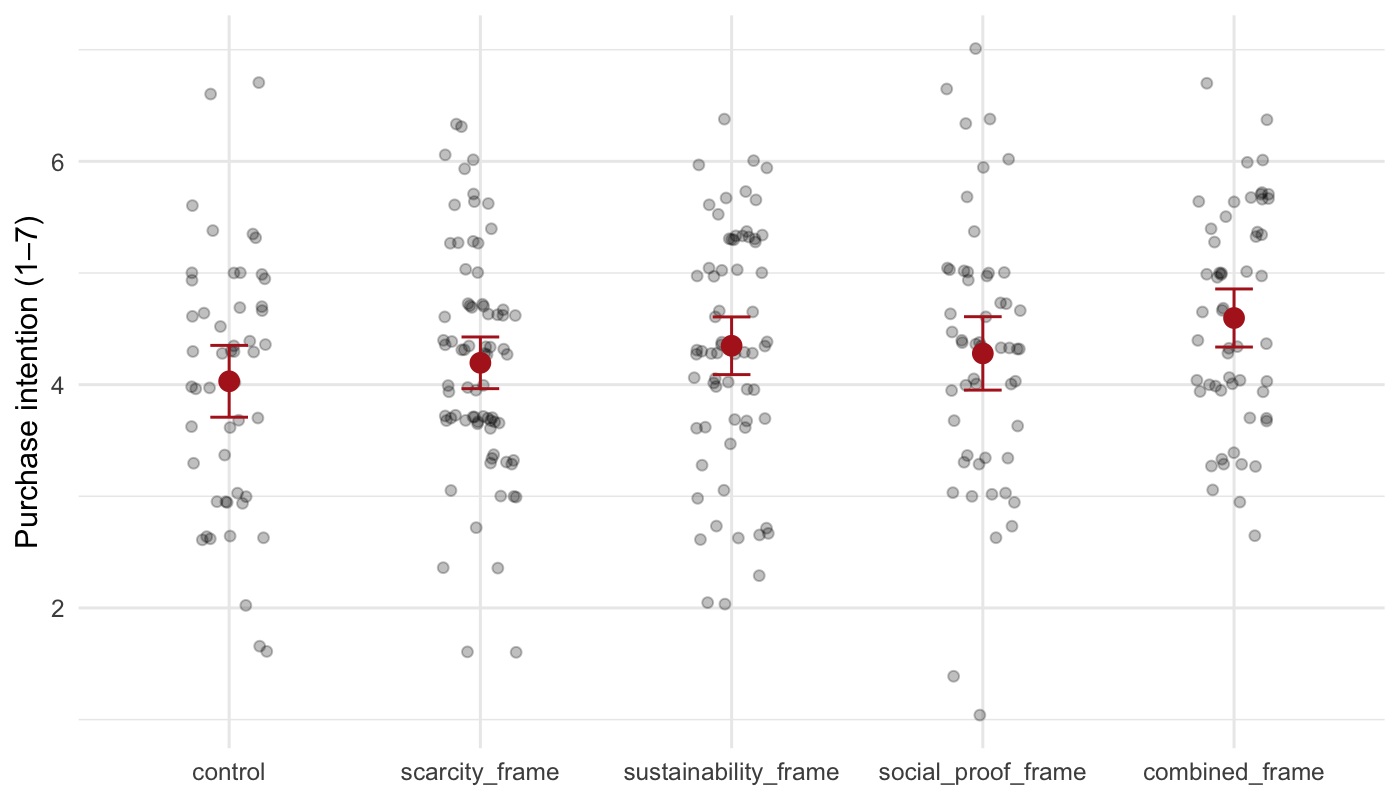
\includegraphics[width=0.85\textwidth]{../figures/fig_01_pi_by_condition.png}
  \caption{Purchase intention by condition. Red points are condition means
           with 95\% confidence intervals.}
  \label{fig:main}
\end{figure}

\subsection{Mediation through perceived value}

\begin{figure}[h]
  \centering
  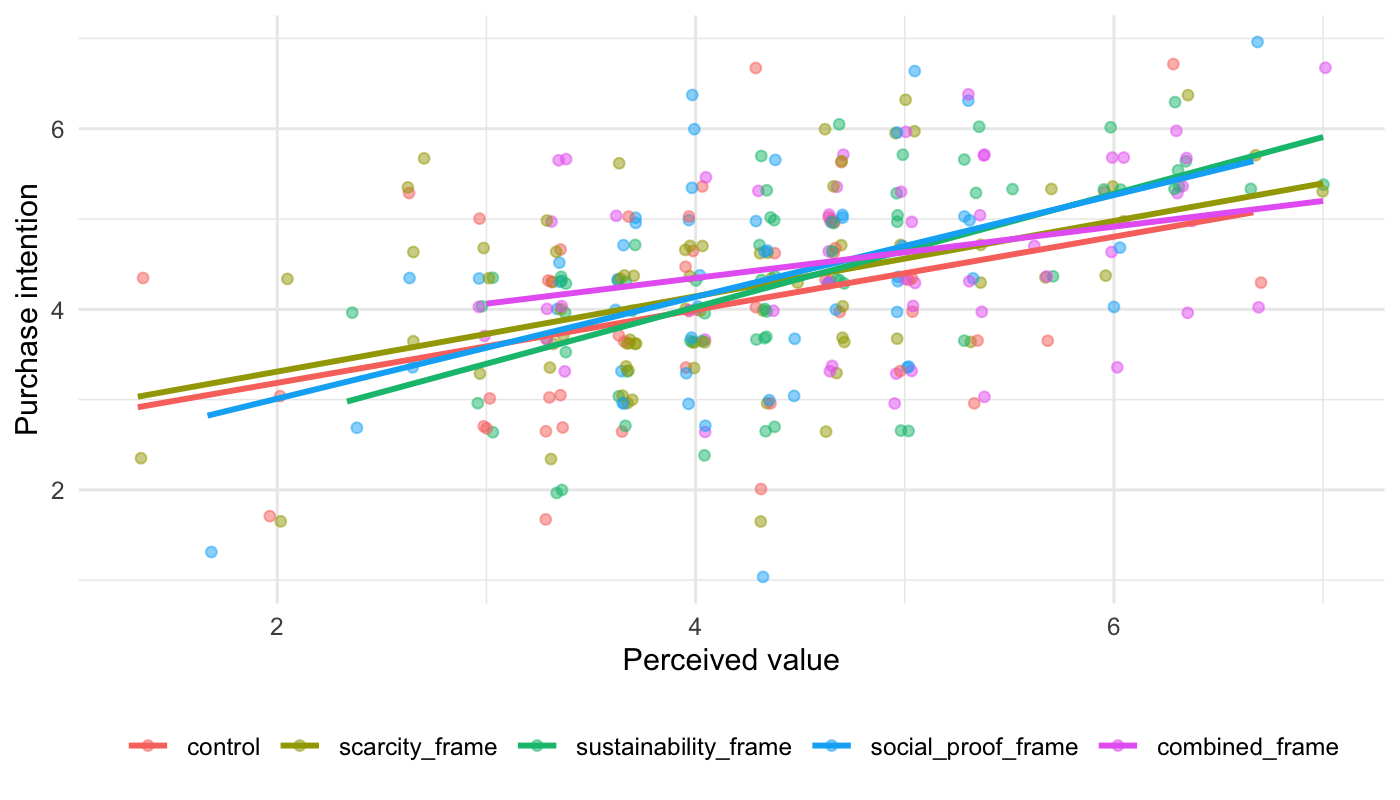
\includegraphics[width=0.85\textwidth]{../figures/fig_02_mediation_scatter.png}
  \caption{Perceived value predicts purchase intention; the conditions
           shift perceived value upward, producing an indirect path.}
  \label{fig:mediation}
\end{figure}

\subsection{Moderation by price sensitivity}

\begin{figure}[h]
  \centering
  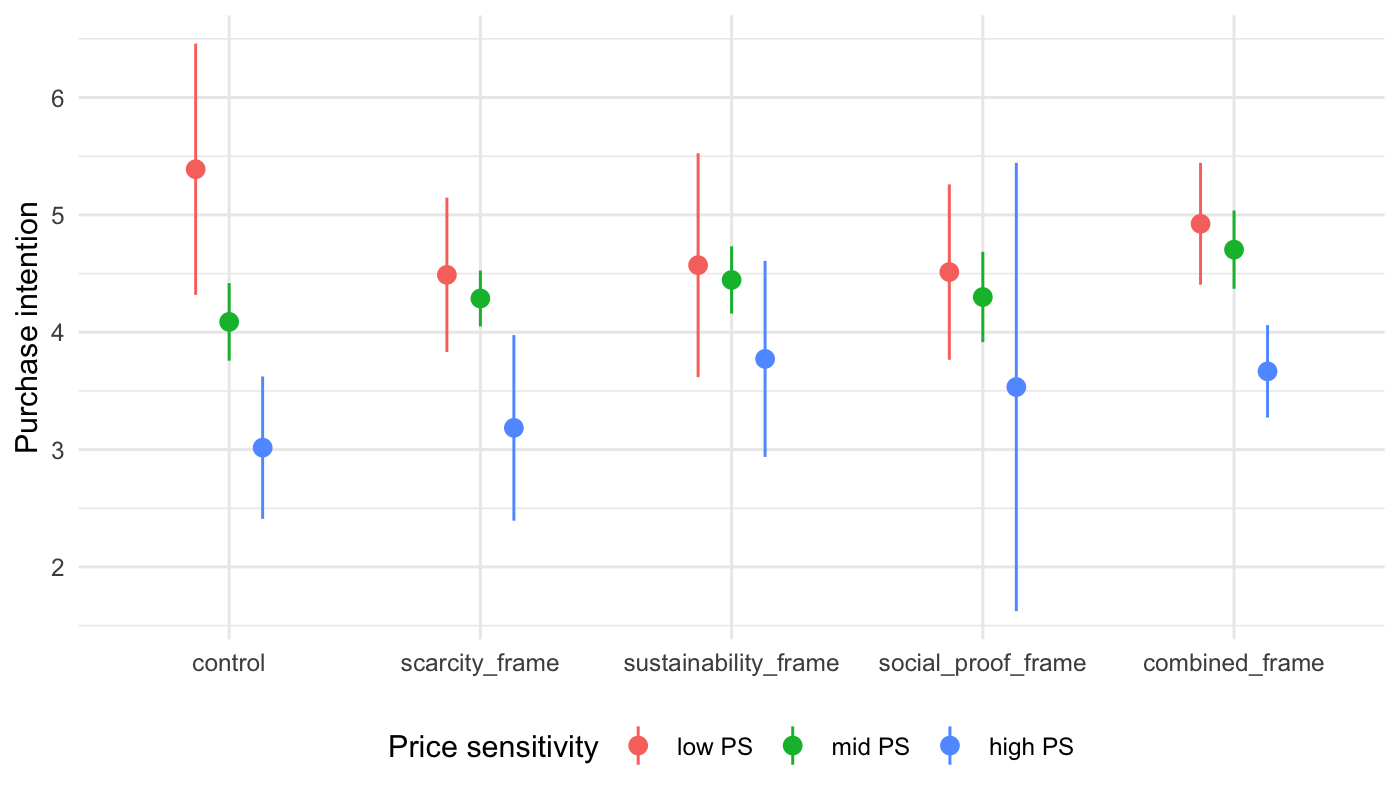
\includegraphics[width=0.85\textwidth]{../figures/fig_03_moderation.png}
  \caption{The condition boost is attenuated for high-price-sensitive
           respondents.}
  \label{fig:moderation}
\end{figure}

\subsection{Model estimates}

Table~\ref{tab:models} collects the coefficients behind the figures above.
It is generated by \texttt{R/03\_analysis.R} and written straight into
\texttt{output/tabs/}, so the numbers in the paper can never drift from the
numbers in the analysis.

\input{output/tabs/model_table.tex}

% sections/discussion.tex — PROSE (no data). Safe to live-edit on Overleaf.
\section{Discussion}

The figures and table referenced above are produced by
\texttt{R/03\_analysis.R}. Re-running that script overwrites them; this
manuscript picks up the new versions on the next compile. No file is
duplicated between code and paper.


% ---- Bibliography ---------------------------------------------------------
\bibliographystyle{plain}
\bibliography{../references/references}

\end{document}
